% Titre : trigo
% Filiere : BCPST
% Difficulte : 
% Type : TD 
% Categories :trigo
% Subcategories : 
% Keywords : trigo




\begin{exercice}  \;
R\'esoudre dans $\R$ les \'equations suivantes et repr\'esenter les solutions sur le cercle trigonom\'etrique:
\begin{enumerate}
\item
$\sin^4{x}+\cos^4{x}=1$
\item
$\sin{\theta}+\sin{(2\theta)}+\sin{(3\theta)}+\sin{(4\theta)}=0$
\item
$\cos{\theta}-\cos{(2\theta)}=\sin{(3\theta)}$
\item
$\cos^3{(x)}\sin{(3x)} + \sin^3{(x)}\cos{(3x)}=\ddp\frac{3}{4}$ \; \textit{(exprimer $\sin{(3x)}$ et $\cos{(3x)}$ 
en fonction de $\sin{x}$ et $\cos{x}$)}
\end{enumerate}
\end{exercice}


\%\%\%\%\%\%\%\%\%\%\%\%\%\%\%\%\%\%\%\%
\%\%\%\%\%\%\%\%\%\%\%\%\%\%\%\%\%\%\%\%
\%\%\%\%\%\%\%\%\%\%\%\%\%\%\%\%\%\%\%\%




\begin{correction}  \;
\begin{enumerate}
 \item \textbf{R\'esolution de $\mathbf{ \sin^4{x}+\cos^4{x}=1 }$:}\\
\noindent 
Le domaine de d\'efinition est $\R$. L'id\'ee ici est de transformer l'\'ecriture afin de factoriser. 
$$\begin{array}{lll}
\sin^4{x}+\cos^4{x}=1 &\Leftrightarrow & \sin^4{x}-1+\cos^4{x}=0
\Leftrightarrow  (\sin^2{x}-1)(\sin^2{x}+1)+\cos^4{x}=0\vsec\\
&\Leftrightarrow & -\cos^2{x}(\sin^2{x}+1)+\cos^4{x}=0
\Leftrightarrow 
\cos^2{x}\left(-\sin^2{x}-1+\cos^2{x} \right)=0\vsec\\
&\Leftrightarrow &  -2\cos^2{x}\sin^2{x}=0
\Leftrightarrow \left\lbrace
\begin{array}{llll}
\exists k\in\Z,& x&=&\ddp\frac{\pi}{2}+k\pi\\
\hbox{ou}\\
\exists k\in\Z,& x&=&k\pi.\\
\end{array}\right.\end{array}$$
\begin{minipage}[c]{0.45\textwidth}
 On obtient donc
$$\fbox{$\mathcal{S}_{\R}=\left\lbrace k\pi,\ k\in\Z \right\rbrace\cup\left\lbrace \ddp\frac{\pi}{2}+k\pi,\ k\in\Z \right\rbrace$}.$$
\end{minipage}
\quad \begin{minipage}[c]{0.45\textwidth}
\begin{center}
\begin{tikzpicture}[scale=2]
%Axes
\draw [->] (-1.1,0) -- (1.1,0);
\draw [->] (0,-1.1) -- (0,1.1);
%Cercle
\draw (0,0) circle (1);
%Points
\draw (1,0) arc (0:90:1) node [red] {$\bullet$};
\draw (1,0) arc (0:90:1) node[above] {$\quad\ddp \frac{\pi}{2}$} ;
\draw (1,0) arc (0:180:1) node [red] {$\bullet$};
\draw (1,0) arc (0:180:1) node[left] {$\ddp \pi\quad$} ;
\draw (1,0) arc (0:270:1) node [red] {$\bullet$};
\draw (1,0) arc (0:270:1) node[below] {$\ddp \ddp\frac{3\pi}{2}\quad$} ;
\draw (1,0) arc (0:0:1) node [red] {$\bullet$};
\draw (1,0) arc (0:0:1) node[right] {$\quad \ddp 0$} ;
\end{tikzpicture}
\end{center}
\end{minipage}
%----------------------------------------------------------
%-------------------------------------------------------------
\item \textbf{R\'esolution de $\mathbf{ \sin{\theta}+\sin{(2\theta)}+\sin{(3\theta)}+\sin{(4\theta)}=0  }$:}\\
\noindent Pour factoriser cette \'equation, il faut utiliser plusieurs fois les formules transformant les sommes en produits.
$$\begin{array}{lll}
\sin{\theta}+\sin{(2\theta)}+\sin{(3\theta)}+\sin{(4\theta)}=0 & \Leftrightarrow & 
\ddp 2 \sin\left(\frac{3\theta}{2}\right) \cos\left(-\frac{\theta}{2}\right) + 2 \sin\left(\frac{7\theta}{2}\right) \cos\left(-\frac{\theta}{2}\right) = 0\vsec\\
& \Leftrightarrow & 
\cos{\left(\ddp\frac{\theta}{2}\right)}\left(\sin{\left(\ddp\frac{3\theta}{2}\right)}+\sin{\left(\ddp\frac{7\theta}{2}\right)}    \right)=0\vsec\\
%& \Leftrightarrow & 
%\sin{\left(\ddp\frac{3\theta}{2}\right)}+\sin{\left(\ddp\frac{7\theta}{2}\right)}=2\sin{\left(\ddp\frac{5\theta}{2}\right)}\cos{\theta}\vsec\\
& \Leftrightarrow & 
\cos{\left(\ddp\frac{\theta}{2}\right)}\sin{\left(\ddp\frac{5\theta}{2}\right)}\cos{\theta}=0\vsec\\
& \Leftrightarrow & 
\left\lbrace\begin{array}{llll}
\exists k\in\Z,& \theta&=&\ddp\frac{2k\pi}{5}\\
\hbox{ou}\\
\exists k\in\Z,& \theta&=&\pi+2k\pi\\
\hbox{ou}\\
\exists k\in\Z,& \theta&=&\ddp\frac{\pi}{2}+k\pi.\\
\end{array}\right.\end{array}$$
\begin{minipage}[c]{0.45\textwidth}
On obtient donc
\conclusion{$\mathcal{S}_{\R}=\left\lbrace \ddp\frac{2k\pi}{5},\ k\in\Z \right\rbrace\cup\left\lbrace \ddp\frac{\pi}{2}+k\pi,\ k\in\Z \right\rbrace\cup\left\lbrace\pi+2k\pi,\ k\in\Z \right\rbrace$}
\end{minipage}

\begin{center}
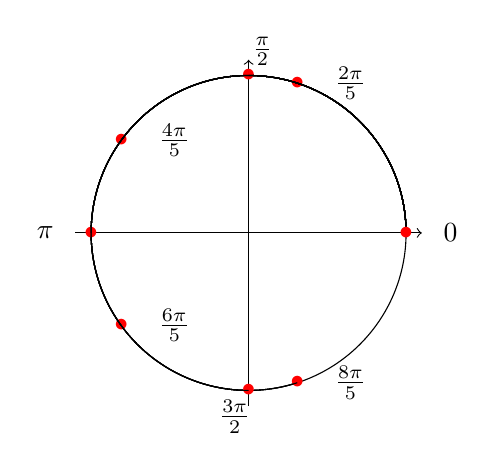
\begin{tikzpicture}[scale=2]
%Axes
\draw [->] (-1.1,0) -- (1.1,0);
\draw [->] (0,-1.1) -- (0,1.1);
%Cercle
\draw (0,0) circle (1);
%Points
\draw (1,0) arc (0:72:1) node [red] {$\bullet$};
\draw (1,0) arc (0:72:1) node[right] {$\quad\ddp \frac{2\pi}{5}$} ;
\draw (1,0) arc (0:144:1) node [red] {$\bullet$};
\draw (1,0) arc (0:144:1) node[right] {$\quad\ddp \frac{4\pi}{5}$} ;
\draw (1,0) arc (0:216:1) node [red] {$\bullet$};
\draw (1,0) arc (0:216:1) node[right] {$\quad\ddp \frac{6\pi}{5}$} ;
\draw (1,0) arc (0:288:1) node [red] {$\bullet$};
\draw (1,0) arc (0:288:1) node[right] {$\quad\ddp \frac{8\pi}{5}$} ;
\draw (1,0) arc (0:180:1) node [red] {$\bullet$};
\draw (1,0) arc (0:180:1) node[left] {$\ddp \pi\quad$} ;
\draw (1,0) arc (0:90:1) node [red] {$\bullet$};
\draw (1,0) arc (0:90:1) node[above] {$\quad\ddp \frac{\pi}{2}$} ;
\draw (1,0) arc (0:270:1) node [red] {$\bullet$};
\draw (1,0) arc (0:270:1) node[below] {$\ddp \ddp\frac{3\pi}{2}\quad$} ;
\draw (1,0) arc (0:0:1) node [red] {$\bullet$};
\draw (1,0) arc (0:0:1) node[right] {$\quad \ddp 0$} ;
\end{tikzpicture}
\end{center}

%------------------------------------------------------------------
\newpage
%-----------------------------------------------------------------
\item  \textbf{R\'esolution de $\mathbf{ \cos{\theta}-\cos{(2\theta)}=\sin{(3\theta)} }$:}\\
\noindent En utilisant tout d'abord les formules transformant les sommes en produits, on obtient
$$\cos{\theta}-\cos{(2\theta)}=-2\sin{\left(\ddp\frac{3\theta}{2}\right)}\sin{\left(-\frac{\theta}{2}\right)}
=2\sin{\left(\ddp\frac{3\theta}{2}\right)}\sin{\left(\ddp\frac{\theta}{2}\right)}.$$
Afin de faire appara\^itre $\sin{\left(\ddp\frac{3\theta}{2}\right)}$ de l'autre c\^ot\'e, ce qui nous permet alors de factoriser, on utilise la formule de duplication des angles et on obtient
$$\sin{(3\theta)}=2\sin{\left(\ddp\frac{3\theta}{2}\right)}\cos{\left(\ddp\frac{3\theta}{2}\right)}.$$
On obtient ainsi
$$\begin{array}{lll}
\cos{\theta}-\cos{(2\theta)}=\sin{(3\theta)}&\Leftrightarrow & 
\sin{\left(\ddp\frac{3\theta}{2}\right)}\left(\sin{\left(\ddp\frac{\theta}{2}\right)}-\cos{\left(\ddp\frac{3\theta}{2}\right)}   \right)=0
\Leftrightarrow 
\left\lbrace\begin{array}{l}
\sin{\left(\ddp\frac{3\theta}{2}\right)}=0\vsec\\
\hbox{ou}\vsec\\
\sin{\left(\ddp\frac{\theta}{2}\right)}=\cos{\left(\ddp\frac{3\theta}{2}\right)}
\end{array}\right.\vsec\\
&\Leftrightarrow & 
\left\lbrace\begin{array}{l}
\sin{\left(\ddp\frac{3\theta}{2}\right)}=0\vsec\\
\hbox{ou}\vsec\\
\sin{\left(\ddp\frac{\theta}{2}\right)}=\sin{\left(\ddp\frac{\pi}{2}-\ddp\frac{3\theta}{2}\right)}
\end{array}\right.
\Leftrightarrow 
\left\lbrace\begin{array}{llll}
\exists k\in\Z,& \theta&=&\ddp\frac{2k\pi}{3}\\
\hbox{ou}\\
\exists k\in\Z,& \theta&=&\pi-3\theta+4k\pi\\
\hbox{ou}\\
\exists k\in\Z,& \theta&=&\pi+3\theta+4k\pi.\\
\end{array}\right.\end{array}$$
\begin{minipage}[c]{0.45\textwidth}
On obtient donc : \vsec\\
\hspace*{-1cm} \fbox{$\mathcal{S}_{\R}=\left\lbrace \ddp\frac{2k\pi}{3},\ k\in\Z \right\rbrace\cup\left\lbrace \ddp\frac{\pi}{4}+k\pi,\ k\in\Z \right\rbrace\cup\left\lbrace -\ddp\frac{\pi}{2}+2k\pi,\ k\in\Z \right\rbrace$}.
\end{minipage}

\begin{center}
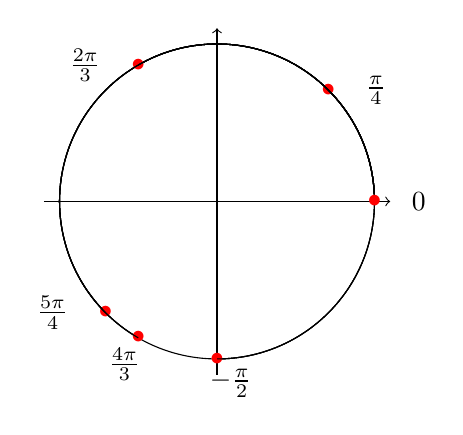
\begin{tikzpicture}[scale=2]
%Axes
\draw [->] (-1.1,0) -- (1.1,0);
\draw [->] (0,-1.1) -- (0,1.1);
%Cercle
\draw (0,0) circle (1);
%Points
\draw (1,0) arc (0:45:1) node [red] {$\bullet$};
\draw (1,0) arc (0:45:1) node[right] {$\quad \ddp \frac{\pi}{4}$} ;
\draw (1,0) arc (0:-90:1) node [red] {$\bullet$};
\draw (1,0) arc (0:-90:1) node[below] {$\quad \ddp - \frac{\pi}{2}$} ;
\draw (1,0) arc (0:225:1) node [red] {$\bullet$};
\draw (1,0) arc (0:225:1) node[left] {$\ddp \frac{5\pi}{4} \quad$} ;
\draw (1,0) arc (0:120:1) node [red] {$\bullet$};
\draw (1,0) arc (0:120:1) node[left] {$ \ddp \frac{2\pi}{3}\quad$} ;
\draw (1,0) arc (0:240:1) node [red] {$\bullet$};
\draw (1,0) arc (0:240:1) node[below] {$\ddp \frac{4\pi}{3}\quad$} ;
\draw (1,0) arc (0:0:1) node [red] {$\bullet$};
\draw (1,0) arc (0:0:1) node[right] {$\quad \ddp 0$} ;
\end{tikzpicture}
\end{center}

%----------------------------------------------------------------------
%----------------------------------------------------------------------
\item \textbf{R\'esolution de $\mathbf{ \cos^3{x}\sin{(3x)}+\sin^3{x}\cos{(3x)}=0 }$:}\\
\noindent
On suit les indications.
\begin{itemize}
 \item[$\bullet$] Expression de $\sin{(3x)}$ en fonction de $\sin{x}$.
$$\begin{array}{lll}
\sin{(3x)}&=& \sin{(2x)}\cos{x}+\sin{x}\cos{(2x)}
= 2\sin{x}\cos^2{x}+\sin{x}\left( 1-2\sin^2{x}  \right)\vsec\\
&=& 2\sin{x}\left(1-\sin^2{x}\right)+\sin{x}-2\sin^3{x}
= -4\sin^3{x}+3\sin{x}.
\end{array}$$
\item[$\bullet$] Expression de $\cos{(3x)}$ en fonction de $\cos{x}$.
$$\begin{array}{lll}
\cos{(3x)}&=& \cos{(2x)}\cos{x}-\sin{(2x)}\sin{x}
= \left(2\cos^2{x}-1   \right)\cos{x}-2\cos{x}\sin^2{x}\vsec\\
&=& 2\cos^3{x}-\cos{x}-2\cos{x}\left( 1-\cos^2{x}  \right)
= 4\cos^3{x}-3\cos{x}.
\end{array}$$
\item[$\bullet$]  R\'esolution.
$$\begin{array}{lll}
\cos^3{x}\sin{(3x)}+\sin^3{x}\cos{(3x)}=0&\Leftrightarrow & \cos^3{x}\left(  -4\sin^3{x}+3\sin{x} \right)+\sin^3{x}\left( 4\cos^3{x}-3\cos{x} \right)=\ddp \frac{3}{4}\vsec\\
&\Leftrightarrow& 3(\sin{x}\cos^3{x}-\sin^3{x}\cos{x})=\ddp \frac{3}{4}\vsec\\
&\Leftrightarrow& \cos{x}\sin{x}\left( \cos^2{x}-\sin^2{x}  \right)=\ddp \frac{1}{4}\vsec\\
\end{array}$$
En utilisant les formules de trigonom\'etrie :
$$\begin{array}{lll}
\cos^3{x}\sin{(3x)}+\sin^3{x}\cos{(3x)}=0&\Leftrightarrow& \ddp \frac{1}{2} \sin{(2x)}\cos{(2x)}=\ddp \frac{1}{4} \; \Leftrightarrow \; \ddp \sin{(4x)}=1\vsec\\
&\Leftrightarrow& \ddp \exists k \in \Z, 4x= \frac{\pi}{2} + 2k \pi\vsec\\
&\Leftrightarrow& \ddp \exists k \in \Z, x= \frac{\pi}{8} + \frac{k \pi}{2}\vsec\\
\end{array}$$
\end{itemize}
\begin{minipage}[c]{0.45\textwidth}
On obtient donc :
$$\fbox{$\mathcal{S}=\left\lbrace \ddp\frac{\pi}{8}+\ddp\frac{k\pi}{2}, k\in\Z \right\rbrace$}.$$
\end{minipage}
\quad \quad \begin{minipage}[c]{0.45\textwidth}
\begin{center}
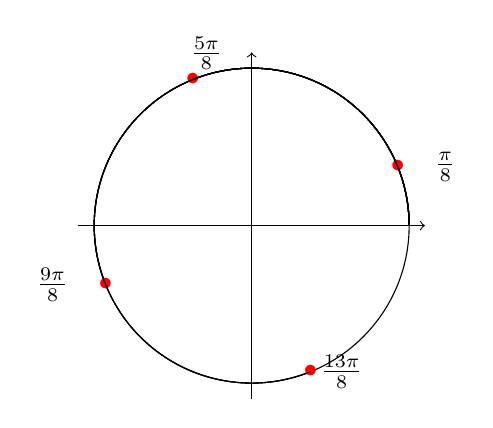
\begin{tikzpicture}[scale=2]
%Axes
\draw [->] (-1.1,0) -- (1.1,0);
\draw [->] (0,-1.1) -- (0,1.1);
%Cercle
\draw (0,0) circle (1);
%Points
\draw (1,0) arc (0:112:1) node [red] {$\bullet$};
\draw (1,0) arc (0:112:1) node[above] {$\quad \ddp  \frac{5\pi}{8}$} ;
\draw (1,0) arc (0:22:1) node [red] {$\bullet$};
\draw (1,0) arc (0:22:1) node[right] {$\quad \ddp \frac{\pi}{8}$} ;
\draw (1,0) arc (0:202:1) node [red] {$\bullet$};
\draw (1,0) arc (0:202:1) node[left] {$\ddp \frac{9\pi}{8}\quad $} ;
\draw (1,0) arc (0:292:1) node [red] {$\bullet$};
\draw (1,0) arc (0:292:1) node[right] {$\ddp \frac{13\pi}{8} \quad$} ;
\end{tikzpicture}
\end{center}
\end{minipage}
\end{enumerate}
\end{correction}